% lec note: https://docs.google.com/document/d/1mhnFaNrPPQxUFme8OVD2Y1bqOOBA-wp7/edit

% lit table: https://docs.google.com/spreadsheets/d/18b49O5U6Iusc4eWiq-ptuGLScmuvRLM1R2cAtGL4iBk/edit#gid=0
% ---------

\section{Chapter Overview}
% 1/4 pg

\section{Problem Domain}
% 3 pgs

The ERC-721 standard implements functionalities to transfer tokens from Blockchain accounts, to get the current token balance of an account, to get the owner of a specific token, the total supply of tokens available on the network, etc. Apart from the item itself, the creator can include metadata such as their signature in the NFT. What began on the Ethereum Blockchain with the ERC-721 standard has since been adopted by other Blockchains. 

% \bigbreak

% Benefits for creators, collectors, buyers
NFTs have a feature to allow a creator to make a certain percentage as royalty whenever the NFT is transferred to a new buyer. Since the items can be verified on the Blockchain, it also ensures that the original creator of the NFT can be tracked down and given due credit, any date in the future, no matter how many wallets it gets passed through \autocite{chevet_blockchain_2018}. Apart from the fact that a buyer can claim the right of ownership of the original item, they also get to financially support the creator. Ultimately, NFTs may gain value over time due to their scarcity. This gives collectors an additional advantage of being able to sell it for a higher price later on.

Creators of NFTs can also create "shares" for their NFT. This allows investors and fans to own a portion of an NFT without having to purchase the entire thing \autocite{noauthor_erc-721_nodate}.

\begin{figure}[h!]
\centering
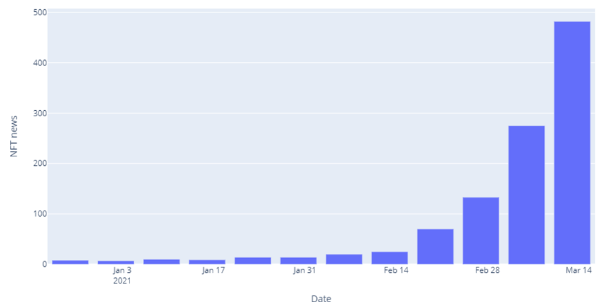
\includegraphics[width=10cm]{NFT-news-trends.png}
\caption{News trend in 2021 related to NFTs \autocite{dowling_fertile_2021}}
\end{figure}

The above figure shows the increase in news trends related to NFTs since the start of 2021. It has been exponentially increasing and hitting headlines around the globe on a daily basis.
This depicts two factors. One is that NFTs are gaining more and more public attraction and acceptance. The second is that since there's a huge buzz among the public on social media and numerous web-sites, it makes sense to consider the opinions that are shared online by them.

% \begin{figure}[h!]
% \centering
% 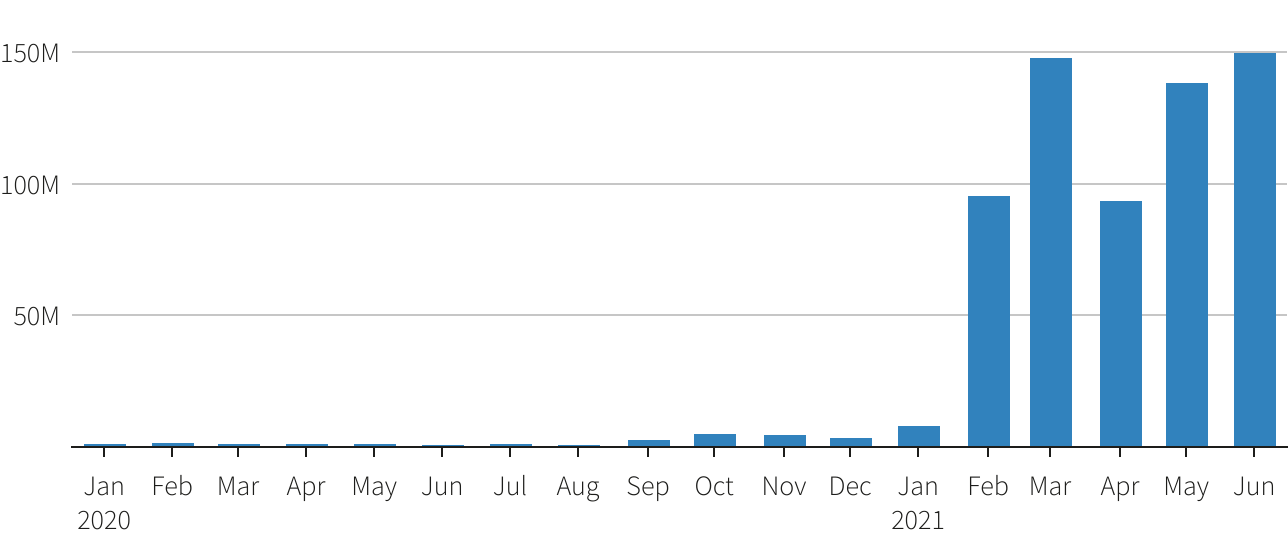
\includegraphics[width=12cm]{images/NFT-sales-opensea.png}
% \caption{Monthly Ethereum-based NFT token sales volume on the OpenSea marketplace, in USD \autocite{howcroft_nft_2021}}
% \end{figure}

% Mention other Blockchains \& marketplaces that sell NFTs
% Market places - OpenSea, Rarible, and Grimes’ choice, Nifty Gateway




% datamining NFTs....
% http://adilmoujahid.com/posts/2021/06/data-mining-meebits-nfts-python-opensea/


% Are Blockchain and AI a Perfect Combination? [WWW Document], n.d. . 101 Blockchains. URL https://101blockchains.com/blockchain-and-ai/ (accessed 7.23.21).


% Add content from 5.2  Understanding factors that affect NFT Markets in proposal


\section{Concept Map}
% 1/4 pg + Appendix

\section{Existing work}
% 4/5pgs+-
% Now it is time to move the Existing work from the proposal to LR (paraphrase it)

There is only one study previously done with related to recommending \gls{nft}s and that study also comes in the form of a blog article on \emph{OpenSea} \autocite{noauthor_what_2020}. The article considers the use of a basic \gls{ml} technique called Multiple Regression with data gathered from OpenSea.


This takes into account previous purchase patterns and NFTs held in wallets to predict whether another wallet carrying a similar combination is likely to own an NFT from a certain category in the future. The categories considered here are mostly collections created by specific well-known creators. Cryptokitties and ENS domains are a couple of examples for collections that have been taken into consideration.

As a final recommendation, this system is capable of presenting NFT categories. Since users can't purchase an entire category, they will have to go back to the process of picking which NFT to purchase in the recommended collection.

This doesn't take into consideration of current global trends and it will not take into account the creators' recognition. An NFT minted by Beeple or a major league like NBA are bound to capture more attention of buyers compared to an NFT minted by a person who hasn't gained any reputation in this space. The major concern with regarding this system is that the user must either enter his preferences manually or provide his wallet key, which holds all of his owned assets, in order to get a recommendation from the system. Although, getting a users' public key can by no means cause any threat of loosing the \gls{nft}s, it can be lead to lack of privacy, which is a tradition that the people into crypto-related assets have a tendancy to be concerned about.


\begin{quote} 
\centering 
\emph{"Crypto has a founding tradition of emphasizing freedom and privacy. Maybe because of this prevailing cultural trend, the NFT space does not have many recommender systems."} 
\\
\raggedleft
\autocite{noauthor_what_2020}
\end{quote}

As mentioned in the same blog post, this tradition is also been identified as a reason to why we have not yet seen much development related to Recommendation Systems in this space. Another reason could be because of the very recent spark in interest this domain has seen in recent times, as mentioned in the Problem Domain.


\bigbreak

A hybrid Recommendations System \autocite{cheng_hybrid_2020} which utilizes opinion \& sentiment extraction techniques from user reviews to create preference profiles for movie recommendations, to enhance the quality of recommendations regardless of the rich or sparse nature of the dataset has been identified as one of the recent researches done towards pushing the limits of baseline recommendation models. The framework that has been designed here uses Collaborative Filtering as the base Recommendations model. The contribution of this research is applicable to the feature engineering stage of the system.

Sentiment analysis is applied on user-reviews to detect user-opinions about movies that were watched and reviewed by users. This data is used to create a user's preference profile, similar to what's created in Content-based filtering. The user's sentiment is identified as a step beyond traditional preference ratings.

% advantages
Due to its capability of dealing with insufficient data, the framework is able to produce recommendations that are more accurate and efficient than existing baseline methods. This proves that using public opinion in the feature engineering stage can enhance the quality of recommendations.

% limitations
Due to the fact that the semantic strategy of opinion extraction being generic, it is understood that it may not be ideal to identify different aspects in varied genres. Examples mentioned are, quality of sound may be of greater interest in action movies, while the story-line in dramas.
Slang, irony \& sarcasm haven't been taken into consideration when extracting user opinion.
A major limitation identified in most systems that rely on similar opinion mining systems is that they are very dependant on the text mining technique used. Another identified drawback in this research by the author is that, to establish a preference profile, a person must have posted reviews on previous movies. If not, those users won't be able to get recommendations. This can be identified as a concern in systems that are dealing with user's who care about their privacy.

\bigbreak

A Deep Belief Network and Sentiment Analysis (DBNSA) has been introduced to achieve data learning for recommendations \autocite{chen_user_2019} to enhance recommendations produced by baseline-recommendation techniques. This deep learning model  processes user comments to generate a possible user rating for user recommendations.

\begin{quote} 
\centering 
\emph{"Users usually transmit their decisions together with emotions."} 
\\
\raggedleft
\autocite{chen_user_2019}
\end{quote}

This research paper emphasizes the necessity of using user comments for recommendation systems since these comments contain a variety of emotional information that can influence the correctness and precision of recommendations.

% >>> feature engineering, pre-processing
Once applying sentiment analysis, a feature vector is created for the input nodes. A noise reduction procedure has been integrated into the system that deletes short comments, comments with no expression and false rating comments. This is used to improve the classification of user ratings. Finally, the DBNSA accomplishes data learning for the recommendations.

% advantages
The paper published claims to outperform baseline models in training loss, precision and recall when tested on Yelp \& Amazon datasets. When tested on the Trip-Advisor dataset, DBNSA had the best \gls{mse} training loss value \& recall. The research also mentions that DBNSA saves more time, while producing results with better accuracy compared to other baseline models.

% limitations
The main drawback that this paper points out is that the proposed system is not suitable \& ready for real-time testing. The authors of the paper have also shown interest in testing the proposed method with a faster Deep Learning algorithm. Similar to the previously mentioned system, sarcastic user-comments have not been taken into consideration here as well.
Out of the two recommendations models that were tested, \emph{libSVM} was identified to have higher accuracy value, \gls{mae} and F-score, while the \gls{mlp} had the highest precision value.

Since user relationships and timeline comments also affect the user's decision making, these can be used to find information from relatable timelines to solve the cold start problem.

\bigbreak
A hybrid approach that combines techniques from content-based filtering, user-to-user collaborative filtering and personalize recommendations \autocite{ayushi_cross-domain_2018} has been introduced to address the limitation of dingle domain analysis. Data sparsity and cold start problem have been pointed out as the addressed limitations. Movie domain knowledge has been used to generate recommendations for books \& music. 
After considering an array of supervised learning algorithms, the authors came to a conclusion that the Decision Tree classifier was found to give the highest accuracy.

% advantages
The use of data from multiple domains allows the system to generate higher accuracy in suggestions. Twitter sentiment has been used to present the user with an analysis of the recommendations produced, to help users in their decision making process.

% limitations
The drawback identified in the Recommendations System developed here is that Twitter sentiment is analysed, calculated and displayed only after showing the user recommendations.The author's suggestion is that only the items with positive sentiment could've been presented, at least results could've been bias towards positive sentiment.

\bigbreak

% ---------- 
Since \gls{nft}s have a distant relationship with crypto assets, it is expected to be of help to understand how crypto assets are evaluated when opted for selection to comprehend how \gls{nft} assets could be evaluated. A study done related to a modelling framework that exposes this area of research \autocite{bartolucci_model_2020} assumes that two main features, namely security and stability can be used to determine the user-desire to own a specific crypto asset. 

Investor's attitudes towards assets’ features, information about the adoption trends, and expected future economic benefits of adoption have been simulated in order to predict the features of the assets that will most likely be adopted. The preference of investors are collected from an app, which calculates the overall state of the 'market'. Then, the app recommends to the user which crypto assets proposed by the user would be a sensible investment. Information about the adoption choice of other investors is considered when making this recommendation.

% limitation
The number of assets, investors and assets' features and investor preferences were fixed within the period of analysis. In a normal use-case scenario, it's highly likely that all these would fluctuate and evolve with the asset's adoption probabilities and expected returns. This revelation clarifies the fact that crypto related assets have a tendency to change with time, social acceptance and trends. Therefore, it is important to consider these factors when building a crypto-related Recommendations System.


% move this to problem solving approaches??
% Lamon, C., Nielsen, E., Redondo, E., n.d. Cryptocurrency Price Prediction Using News and Social Media Sentiment 6.

% (-)Abraham, J., Higdon, D., Nelson, J., Ibarra, J., 2018. Cryptocurrency Price Prediction Using Tweet Volumes and Sentiment Analysis 1, 22.
% ***his has why sentiment analysis isn't that important
% paraphrase quotes from this paper.

% While some studies present various methods to analyse news and social media sentiment, especially with the use of Twitter & Google Trends \autocite{},  

% ---------- 

% *** add a summary of all discussed systems here??



\bigbreak
% move this to problem solving approaches??
% ---------- Price Prediction models

%  This para might be better-suited under Problem Domain
When considering ownership desire of \gls{nft}s, it is understood from domain research that the increase in price of an \gls{nft} has the possibility of being a factor to be considered when making a purchase.
%  *** cite literature that tells NFTs behaviour compared to crypto - can be cited under Problem Domain as well
As mentioned under the Problem Domain section of this literature review, it is understood that \gls{nft}s have very little spill-over with other Crypto assets. However, knowing Crypto price prediction models is important since Wavelet coherence analysis indicates a co-movement between these two markets \autocite{dowling_is_2021}.
These models can be used separately on each NFT asset to anticipate the pricing with related to time, sales \& bids.
The author finds this research to be related to address the research gap in this thesis since an appropriate price prediction could be used to enhance \Gls{nft}  recommendations to users.

Past research suggests a model which employs time series techniques, can predict the price for the next few days by splitting the data into train and test runs \autocite{ferdiansyah_lstm-method_2019}.

% limitations
In terms of RMSE (Root Mean Squared Error), the result is insufficient. The authors of this research have shown interest in testing out this method with modified \gls{lstm} layers by adding dropout and modifying the number of epochs. Using different instability data-sets can also be tried out to test how good the prediction results could get. 
Furthermore, sentiment analysis is also proposed as future work to be combined with the \gls{lstm} method. This could be used to identify how public sentiment 'causes the value of crypto to adjust, with related to past price-fluctuations.


\subsection{Benchmarking}
% 1
% *** make a table on MSE, MAE, P@K, etc and explain what they test - cite


% ***cite & explain: the difficulty in benchmarking recommendation systems paper



% Since the only work related to an NFT Recommendation System does not have a specific measure of benchmarking, the \gls{p@k} measurement can be used for this purpose as well as \gls{mse}
% can evaluation and benchmarking be the same?



\section{Review of Different Problem-solving Approaches}
% unused technologies in domain can come here as well.
% 4pgs+-
There are several baseline techniques of Recommendations Systems that have been used by the biggest data-driven companies around the world.
% Explain about Collaborative, Content-based Filtering, Hybrid, Deep Learning Techniques, drawbacks, why baseline methods should be pushed forward using feature engineering, etc.


\bigbreak
\autocite{larry_history_2019}
% move this to problem solving approaches?
% *** describe
% use this to explain in Benchmarking/ Evaluation approaches as well (can speak about P@K measurement and top N strategy?)
There have been many attempts to expand the capabilities of Recommendations by making use of public opinion. Collaborative Filtering was one approach to achieve that. Another identified approach was to make use of user-data on social media. This has been integrated into Machine Learning-based Hybrid Recommendation Architectures in many ways. In recent research done by Amazon \autocite{larry_history_2019} it is understood that when a timeline is considered for recommendations, an \emph{Autoencoder} Deep Learning model is capable of Recommending the best possible combination of movies to users.

% LSTM? for predictions

% NLP techniques that can be applied (Sentiment analysis, word/ noun matching)

\section{Review of Evaluation Approaches}
%  (quantitative or qualitative)
% 4pgs+-


\section{Tools}
% 3/4pgs+-


\section{Chapter Summary}
% 1/2 pg